\documentclass{sig-alternate}
\usepackage{multirow}
\usepackage{color}
\usepackage{colortbl}
\usepackage{picture}
\usepackage{algorithm}
\usepackage{algorithmicx}
\usepackage{algpseudocode}
\renewcommand{\algorithmicrequire}{\textbf{Input:}}
\renewcommand{\algorithmicensure}{\textbf{Output:}} 
\newcommand{\lucas}[1]{\textcolor{red}{#1}} 
\newcommand{\bill}[1]{\textcolor{blue}{#1}} 
\newcommand{\carter}[1]{\textcolor{cyan}{#1}} 
%\newenvironment{changed}{\par}{\par}

%timm tricks
\newcommand{\bi}{\begin{itemize}[leftmargin=0.4cm]}
\newcommand{\ei}{\end{itemize}}
\newcommand{\be}{\begin{enumerate}}
\newcommand{\ee}{\end{enumerate}}
\newcommand{\tion}[1]{\S\ref{sect:#1}}
\newcommand{\fig}[1]{Figure~\ref{fig:#1}}
\newcommand{\eq}[1]{Equation~\ref{eq:#1}}
 

\usepackage[shortlabels]{enumitem} 
\usepackage{times}
\newcommand{\subparagraph}{}
\usepackage{url}
\def\baselinestretch{1}


\setlist{nosep}
 \usepackage[font={small}]{caption, subfig}
\setlength{\abovecaptionskip}{1ex}
 \setlength{\belowcaptionskip}{1ex}

 \setlength{\floatsep}{1ex}
 \setlength{\textfloatsep}{1ex}
\usepackage[compact,small]{titlesec}
\DeclareMathSizes{7}{7}{7}{7} 
\pagenumbering{arabic}
\setlength{\columnsep}{7mm}

\begin{document}

\conferenceinfo{FSE}{'15 Bergamo, Italy}
\title{Revisiting the Truisms of Software Engineering:\\ Does Phase Delay Exponentially Increases  Repair Time?}
\numberofauthors{3}
\author{
\alignauthor
Tim Menzies, \\Carter Pape\\
       \affaddr{CS, NcState, USA}\\
       tim.menzies@gmail.com,\\carterpape@gmail.com
\alignauthor
William Curtis,\\ Forrest Schull\\
\affaddr{SEI, CMU, USA}
wrn,fjshull@sei.cmu.edu
\alignauthor
Lucas \\Layman\\
       \affaddr{Fraunhofer Center,  USA}\\ 
       llayman@fc-md.umd.edu
} 


 
\maketitle
\begin{abstract}
Does
repair time increases exponentially
the longer a defect persists in a system?
This  is very widely belief and the core rational  for
 rejecting   traditional linear development methods
 in favor of more cyclic agile approaches.

This paper shows that this belief is maintained
quite strongly in the industrial software engineering
community (but, in the academic community, somewhat less so).
Yet based on a sample of 
\carter{230} software projects from around the world from 
\bill{2005 to 2013}, we argue that this belief is mostly 
incorrect. Specifically: the median fix time for issues
is just a few minutes and this increases by a small linear amount
the longer the issue remains in the system. 

What was observed was a small number
of defects that take a remarkably long time to resolve
For these issues, if an issue takes more an hour
to resolve then it will usually require many more hours of work.
These long-tail bugs
are more prevalent the longer a project delays issue removal. 
In order to handle such ``long tail'' issues,
we suggest  augmenting software
development groups with additional ``tiger teams'' that are triggered
when issue resolution time increases beyond a certain number of
minutes.
\end{abstract}

% A category with the (minimum) three required fields
\vspace{1mm}
\noindent
{\bf Categories/Subject Descriptors:} 
D.2.8 [Software Engineering]: Product metrics; 

 

\vspace{1mm}
\noindent
{\bf Keywords:} defect prediction, 

\section{Introduction}
Several recent papers call into questions long-held trusims in the field
of software engineering. Devanbu reports that, in practice, the advantage of types languages
is only very minimal. Nagappan et al. found that XXX, contrary to the advice of Dyketra,
it is not necessarily true that ``goto considered harmful'' XXX. More generally,
several recent  papers comment on ``locality'' effects where effects
thold  generally across XXXX
 
Perhaps it is time to take a look at the base premises of our field, particularly in light of the large software analytics data sets newly available for reseaercehrs.

XXX tsp. 40MB . 235 prokects

\section{Related Work}

In their text Romabach laws

Kent Beck's original extreme programming text is big on this.

Historical  evidence for this dataes back to some studies in the 1970s. To the best of
our knowledge, not updated since. Regardless, as discussed in the next section, this

The first data on the cost to fix defects as a function of lifecycle phase date back to large systems in the late 70s from IBM~\cite{Fagan76}, TRW~\cite{Boehm76}, GTE~\cite{Daly77}, and Bell Labs~\cite{Stephenson76} (Figure~\ref{fig:cost-to-fix}). These studies suggest that the cost (in terms of effort) to find and fix an error monotonically increases with lifecycle phase. For large projects, the ratio of cost-to-fix in the requirements phase to cost-to-fix in operation is on the order of 1:100. Furthermore, cost function is superlinear, with the greatest rates of increase in the acceptance testing and operations phases.

\begin{figure}[!ht]
 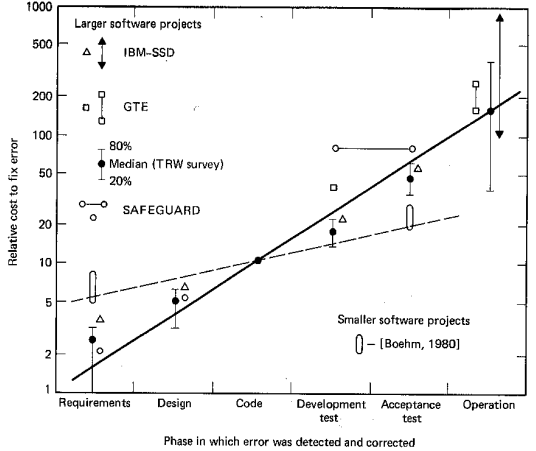
\includegraphics[width=3.3in]{boehm_cost-to-fix.png}
 \caption{Historical cost-to-fix curve. From~\cite{Boehm81}.}\label{fig:cost-to-fix}
 \end{figure}
 
In the 40 years since these initial studies, few studies have been published on the cost-to-fix curve as a function of lifecycle phase. Boehm~\cite{Boehm80} provides data suggesting that the cost-to-fix curve for small projects (from two student projects of 2000 deliverable source instructions) is flatter than for large projects (the dashed line of Figure~\ref{fig:cost-to-fix}). Shull et al.~\cite{Shull02} conducted a literature survey and held a series of e-workshops with industry experts on fighting defects. Workshop participants from Toshiba and IBM reported cost-to-fix ratios of 1:137 and 1:117 for large projects respectively~\cite{Shull02} -- the raw data points are not provided. One notable example to the traditional cost-to-fix curve is the CCPDS-R described by Royce~\cite{Royce98}: a million-line, safety-critical missile defense system (Figure~\ref{fig:royce}). In this project, design changes (including architecture changes) required approximately twice the effort of implementation and test changes, and the cost-to-fix in implementation and test phases increased slowly. Boehm~\cite{Boehm10} attributes this success to the CCPDS-R development process, which focused on removing architecture risk early in the development lifecycle.

\begin{figure}[!ht]
 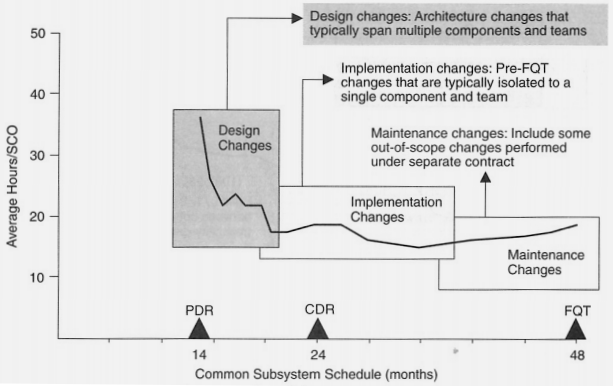
\includegraphics[width=3.3in]{Royce98.png}
 \caption{Exception to the rule - CCPDS-R case study cost-to-fix curve. From~\cite{Royce98}.}\label{fig:royce}
 \end{figure}
 
As discussed is \S\ref{sec:why-study}, one goal of agile methods is to flatten the cost-to-change curve~\cite{beck00}. Relatively little empirical data exists on this point. Clutterbuck et al.~\cite{Clutterbuck09} studied 5-month effort by a small-to-medium enterprise team developing a 71KLOEC web interface to a database application to implement 18 change requests (Figure~\ref{fig:clutterbuck}). Note that these were for new and changed user requirements, not defects. Clutterbuck et al. found the cost of change to be relatively flat until the later phases, with much of the effort spent in analysis of the change requests~\cite{Clutterbuck09}. Elssamadisy and Schalliol~\cite{Elssamadisy02} anecdotally report on the growing, high cost of rework in a 50 person, three-year, 500KLOEC Extreme Programming project as the project grew in size and complexity.

\begin{figure}[!ht]
 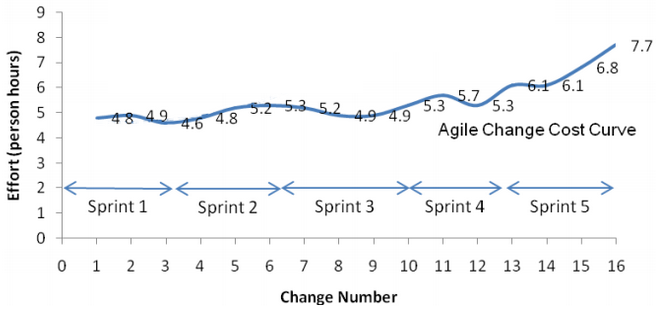
\includegraphics[width=3.3in]{clutterbuck.png}
 \caption{Cost of change from an agile case study. From~\cite{Clutterbuck09}.}\label{fig:clutterbuck}
 \end{figure}
 
 We note that previous work focuses on cost-to-fix as a function of lifecycle phase irrespective of when the defect was injected, that is, previous work analyzes the cost to fix a defect found in test regardless of whether that defect was a requirements error or a coding mistake. To our knowledge, our research represents the first large-scale study of phase delay.

\section{lucasSurvey}






Our survey collected data on software engineers' views of commonly held software engineering ``laws''.
One of the laws questioned relates directly to phase delay: ``Requirements errors are the most expensive to fix when found during production but the cheapest to fix early in development'' (from Glass~\cite{glass02} p.71 who references Boehm \& Basili~\cite{boehm01}). We abbreviate this law as RqtsErr. 

The survey was conducted in two phases using Amazon's Mechanical Turk. The first phase was conducted only with professional software engineers solicited through the Mechanical Turk\footnote{Professional software engineers were required to complete a pretest to verify their status as a professional or open source software developer and to confirm their knowledge of basic software engineering terminology and technology.}, and the second survey was conducted Program Committee members of the ESEC/FSE and ICSE conferences solicited via email.

The respondents answered the following questions for the laws they were presented: \newline
\textbf{Agreement:} ``Based on your experience, do you agree that the statement above is correct?'' A Likert scale captured the agreement score from Strongly Disagree to Strongly Agree. A text box was provided to explain the answer. \newline
\textbf{Applicability:} ``To the extent that you believe it, how widely do you think it applies among software development contexts?'' The possible answers were presented as a scale from -1 to 5:
\begin{itemize}
\item I don't know (-1)
\item This law does not apply at all (0)
\item Applies in a very narrow range of projects  (1)
\item Rarely applies (2)
\item Occasionally applies (3)
\item Very frequently applies (4)
\item Always applies (5)
\end{itemize}
Respondents were required to explain the applicability score in a text box.

Participants were presented with the RqtsErr law and others drawn from \cite{glass02} and \cite{endres03}. The PC member survey contained an additional question on ``In general, the longer errors are in the system (requirements errors, design errors, coding errors, etc.), the more expensive they are to fix'' (PhaseDelay for short). Responses were recorded using the Agreement question Likert scale. 

Summary statistics for the agreement and applicability scores for the RqtsErr and PhaseDelay laws are presented in Figure~\ref{fig:survey_results}. Responses whose Applicability response was ''I don't know'' are ommitted from analysis.


\begin{figure}[!ht] 
\scriptsize
\begin{center}
\subcaption{Practitioner survey}
\begin{tabular}{l|c|c|c|c|c}
Law & N & \multicolumn{2}{c}{agreement} & \multicolumn{2}{c}{applicability} \\ 
 & & $\bar{x}$ & $\tilde{x}$ & $\bar{x}$ & $\tilde{x}$ \\
\hline 
\textbf{Rqts errors are most expensive...} & 16 & 4.6 & 5 & 4.2 & 4 \\ 
Process maturity improves output & 17 & 4.4 & 4 & 3.9 & 4 \\ 
Most time is spent removing errors & 16 & 4.1 & 4 & 3.9 & 4 \\ 
Missing reqts are hardest to fix & 17 & 4.1 & 4 & 4.0 & 4 \\
Reuse increases prod. and qual. & 16 & 3.9 & 4 & 3.8 & 4 \\
OO-programming reduces errors & 13 & 3.9 & 4 & 3.5 & 4 \\
80-20 rule (defects to modules) & 12 & 3.8 & 4 & 4.0 & 4 \\
Adding manpower to a late project & 15 & 3.7 & 4 & 3.7 & 4 \\
Inspections can remove 90\% of defects & 18 & 3.3 & 4 & 3.5 & 4 \\
Smaller changes have higher error density & 14 & 2.8 & 3 & 3.4 & 3.5 \\
A developer is unsuited to test own code & 17 & 2.6 & 3 & 3.5 & 4
\end{tabular} 
\bigskip
\subcaption{Researcher survey}
\begin{tabular}{l|c|c|c|c|c}
Law & N & \multicolumn{2}{c}{agreement} & \multicolumn{2}{c}{applicability} \\ 
 & & $\bar{x}$ & $\tilde{x}$ & $\bar{x}$ & $\tilde{x}$ \\
\hline 
Process maturity improves output & 4 & 4.0 & 4 & 4.0 & 4 \\
\textbf{Rqts errors are most expensive...} & 30 & 3.8 & 4 & 3.8 & 4   \\ 
80-20 rule (defects to modules) & 6 & 3.7 & 4 & 3.5 & 4 \\
\textbf{PhaseDelay} & 30 & 3.6 & 4 & -- & --  \\ 
Missing reqts are hardest to fix & 7 & 3.6 & 4 & 3.7 & 4 \\
Adding manpower to a late project & 4 & 3.5 & 4 & 3.5 & 4 \\
Inspections can remove 90\% of defects & 7 & 3.4 & 4 & 3.6 & 3 \\
Reuse increases prod. and qual. & 6 & 3.3 & 4 & 3.0 & 4 \\
OO-programming reduces errors & 6 & 3.2 & 4 & 2.7 & 3 \\
Most time is spent removing errors & 6 & 2.8 & 3 & 3.2 & 4 \\ 
Smaller changes have higher error density & 4 & 2.8 & 3 & 4.0 & 4 \\
A developer is unsuited to test own code & 7 & 2.1 & 2 & 2.4 & 3
\end{tabular} 

\end{center}
\caption{Agreement and applicability of software engineering axioms.}
\label{fig:survey_results}
\end{figure}

While the practitioners strongly believed in the law, researchers were less firm. In the free response texts, most participants agreed that addressing errors late may mean system redesign unless the system and the affected requirement are simple/trivial. Further, any changes to the production system have additional complexity (compared to changes while system in development) due to users, data existence, and architecture dependencies. The researchers who disagreed with the law generally asserted that requirements change can be expensive, but that depends on the process used (e.g., agile vs. waterfall) and the adaptability of the system architecture.

Overall, the RqtsErr law was the most agreed upon and most applicable law of 11 surveyed amongst practitioners, and the second most agreed upon law amongst researchers. The survey results seem to confirm that the notion that phase delay escalates cost-to-fix is a widely-held belief in software engineering.


\section{billTSP}

\section{carterCharts}

anything

\sction{Data}

\begin{figure}[!t]

%\renewcommand{\baselinestretch}{0.8}
\scriptsize
\begin{center}
\begin{tabular}{r|rrr|ll}
  Sample&\multicolumn{3}{c|}{Percentiles}\\ 
size & 25th & 50th & 75th & Phase injected & Phase removed\\\hline
57& 6& 16& 47&  BeforeDevelopment&Code\\
72& 2& 4& 11&  BeforeDevelopment&CodeInspect\\
165& 6& 18& 56&  BeforeDevelopment&Test\\
50& 6& 20& 37&  BeforeDevelopment&IntTest\\
42& 8& 28& 65&  BeforeDevelopment&SysTest\\\hline

66& 2& 6& 15&  Planning&Planning\\
41& 1& 5& 16&  Planning&ReqtsReview\\\hline

23& 0& 1& 3&  Reqts&Reqts\\
245& 6& 13& 23&  Reqts&ReqtsReview\\
289& 7& 16& 30&  Reqts&ReqtsInspect\\
32& 6& 21& 40&  Reqts&Design\\
49& 2& 7& 24&  Reqts&DesignInspect\\\hline
 

94& 2& 5& 10&  HLD&HLDReview\\
133& 3& 8& 19&  HLD&HLDInspect\\
33& 2& 5& 17&  HLD&Design\\\hline



37& 2& 4& 6&  Design&Design\\
455& 11& 24& 53&  Design&DesignInspect\\
218& 5& 14& 30&  Design&Code\\
166& 4& 11& 22&  Design&CodeInspect\\
542& 14& 31& 60&  Design&Test\\
67& 6& 15& 40&  Design&IntTest\\
92& 10& 25& 53&  Design&SysTest\\\hline

53& 2& 4& 9&  DesignInspect&DesignInspect\\
38& 1& 3& 9&  DesignInspect&Code\\\hline

126& 4& 12& 31&  Code&Code\\
459& 11& 24& 45&  Code&CodeInspect\\
461& 11& 26& 55&  Code&Test\\
348& 10& 26& 62&  Code&IntTest\\
230& 8& 18& 39&  Code&SysTest\\
71& 2& 11& 28&  Code&AcceptTest\\\hline

64& 2& 4& 10&  CodeInspect&CodeInspect\\
57& 2& 5& 13&  CodeInspect&Test\\\hline



110& 3& 10& 23&  Test&Test\\
66& 2& 4& 12&  Test&QualTest\\\hline


32& 1& 2& 4&  IntTest&QualTest\\
36& 1& 11& 30&  IntTest&IntTest\\
21& 1& 2& 5&  IntTest&SysTest\\
 \end{tabular}
\end{center}
\caption{Distribution of fix times seen in SEI TSP data.}
\label{fig:faw}
\end{figure}
 
 
\begin{figure}
\begin{center}
\scriptsize
\begin{tabular}{rrl}
year& \# issues&\\\hline
2006 &  44 &\\
2007 &  34 &\\
2008&  288 &\rule{1mm}{2mm}\\
2009&  846 &\rule{3mm}{2mm}\\
2010& 1007 &\rule{3mm}{2mm}\\
2011& 3273 &\rule{10mm}{2mm}\\
2012&18102 &\rule{45mm}{2mm}\\
2013&20336 &\rule{50mm}{2mm}\\
2014& 3307 & \rule{10mm}{2mm}\\\cline{1-2}
Total:&47228
\end{tabular}
\end{center}
\caption{This paper studies 47,228 issues recorded 2006 to 2014.}\label{fig:years}
\end{figure}
\begin{figure*}
\begin{center}
\includegraphic[width=6in]{waterfall.png}
\end{center}
\caption{Some parts of the waterfall cycle.}
\end{figure*}
\begin{figure}
\begin{center}
\includegraphic[width=3.5in]{agile.png}
\end{center}
\caption{Some parts of the waterfall cycle.}
\end{figure}

\begin{figure*}[!t]

\renewcommand{\baselinestretch}{0.7}
\small
\begin{center}
\begin{tabular}{ll|r|rl}
            &                  & Sample\\
Phase injected & Phase removed & size & \multicolumn{2}{l}{Scale up, w.r.t. to first phase}
\\\hline

BeforeDevelopment&Code.dat&57&1&\rule{2mm}{2mm} \\
BeforeDevelopment&CodeInspect.dat&72&0.3&\rule{0mm}{2mm} \\
BeforeDevelopment&Test.dat&165&1.1&\rule{2mm}{2mm} \\
BeforeDevelopment&IntTest.dat&50&1.3&\rule{2mm}{2mm} \\
BeforeDevelopment&SysTest.dat&42&1.8&\rule{2mm}{2mm} \\
\\\hline

Planning&Planning.dat&66&1&\rule{2mm}{2mm} \\
Planning&ReqtsReview.dat&41&0.8&\rule{0mm}{2mm} \\
\\\hline

Reqts&Reqts.dat&23&1&\rule{2mm}{2mm} \\
Reqts&ReqtsReview.dat&245&13&\rule{26mm}{2mm} \\
Reqts&ReqtsInspect.dat&289&16&\rule{32mm}{2mm} \\
Reqts&Design.dat&32&21&\rule{42mm}{2mm} \\
Reqts&DesignInspect.dat&49&7&\rule{14mm}{2mm} \\
\\\hline
 

HLD&HLDReview.dat&94&1&\rule{2mm}{2mm} \\
HLD&HLDInspect.dat&133&1.6&\rule{2mm}{2mm} \\
HLD&Design.dat&33&1&\rule{2mm}{2mm} \\
\\\hline

Design&Design.dat&37&1&\rule{2mm}{2mm} \\
Design&DesignInspect.dat&455&6&\rule{12mm}{2mm} \\
Design&Code.dat&218&3.5&\rule{6mm}{2mm} \\
Design&CodeInspect.dat&166&2.7&\rule{4mm}{2mm} \\
Design&Test.dat&542&7.7&\rule{14mm}{2mm} \\
Design&IntTest.dat&67&3.7&\rule{6mm}{2mm} \\
Design&SysTest.dat&92&6.3&\rule{12mm}{2mm} \\
\\\hline

DesignInspect&DesignInspect.dat&53&1&\rule{2mm}{2mm} \\
DesignInspect&Code.dat&38&0.75&\rule{0mm}{2mm} \\
\\\hline

Code&Code.dat&126&1&\rule{2mm}{2mm} \\
Code&CodeInspect.dat&459&2&\rule{4mm}{2mm} \\
Code&Test.dat&461&2.16667&\rule{4mm}{2mm} \\
Code&IntTest.dat&348&2.16667&\rule{4mm}{2mm} \\
Code&SysTest.dat&230&1.5&\rule{2mm}{2mm} \\
Code&AcceptTest.dat&71&0.916667&\rule{0mm}{2mm} \\
\\\hline

CodeInspect&CodeInspect.dat&64&1&\rule{2mm}{2mm} \\
CodeInspect&Test.dat&57&1.25&\rule{2mm}{2mm} \\
\\\hline

Test&Test.dat&110&1&\rule{2mm}{2mm} \\
Test&QualTest.dat&66&0.4&\rule{0mm}{2mm} \\
\\\hline

IntTest&QualTest.dat&32&1&\rule{2mm}{2mm} \\
IntTest&IntTest.dat&36&5.5&\rule{10mm}{2mm} \\
IntTest&SysTest.dat&21&1&\rule{2mm}{2mm} \\ 
\end{tabular}
\end{center}
\caption{Scale ups for median time to resolve issues (taken from \fig{raw}).}
\label{fig:scale}
\end{figure*}

The starting point for this paper were the times required to fix 47,228 issues.
All data was collected
by the Software Engineering Institute in the period 2006 to 2014 (see \fig{years}).
To the best of our knowledge, this is the largest sample of ``time to fix issues''
yet analyzed. 

This data was collected using the   methodology described by
Watts Humphrey's Team Software Process~\cite{tsp00}. TSP is an extension of Humphrey's early
work on Personnel Software Process~\cite{psp05}.  PSP encourages developers to continually make estimates
about their day-to-day tasks, then compare those estimates against the actual development effort
(in this way, developers can acquire a more realistic understanding of their work behaviour).

In all data, was collected from 172 separate projects. Given Beck's comments (above) about phase delay motivating agile processes, we take care to identify the differences of these 
projects to agile development projects. In what we call a ``standard agile'' project, there exists
some backlog of tasks. When teams complete their current tasks, they reach into to the backlog
to select the next task(s) to complete. That selection process may use a variety of criteria
to prioritize which  tasks are selected (for more details on that selection process, see~\cite{me09j,port08,boehmturner03}). Tasks are completed in ``sprints'' that can last hours,
days, but rarely not more than weeks. Each day meet for brief ``scrum'' sessions to assess (and possibly alter) their current progress on the goals of the spring.  

One way to characterize the above is a ``micro cyclic'' approach where teams 
constantly reassess their priorities using feedback gained after trying to code 
functionality X,Y,Z. An alternate, more traditional approach is a ``macro linear''
approach such as the ``waterfall methodology'' that develops code after an extensive
pre-planning stage:

\[
\mathit{Reqts}
\mathit{ReqtsReview}
\mathit{ReqtsInspect}

\mathit{HighLevelDesign}
\mathit{HighLevelReview}
\mathit{HighLevelInspect}

\mathit{Design}
\mathit{DesignReview}
\mathit{DesignInspect}

\mathit{Code}

\mathit{Compile}
\mathit{Test}
\mathit{IntTest}
\mathit{SysTest}
\]

In the original paper defining and 
critiquing ``waterfall'', Royce defines a set of assessment and feedback processes
such that 


care to contrast these 
The majority of the teams follow a basically linear process within a single feature of physical component (usually no more than a week or two work in total). Unlike some agile teams, *most*TSP teams will not conflate development and unit test.  This is usually pretty clear from the task  phase sequencing. A few teams choose to follow a Test Driven Development like process in which code review or inspection will follow test. In a more traditional “micro-linear” TSP approach, unit test follows inspections. 


Our data reporting the time required
to resolve issues in phase $j$ that there were introduced in phase $i, i<j$.



The defect typ that we studied were
\be 
\item design, compile, test, or other support system problems = Environment
procedure calls and reference, I/O, user formats = Interface
structure, content = Data
comments, messages = Documentation
spelling, punctuatio typos, instruction formats = Syntax
logic, pointers, loops, recursion, computation, function defects = Function
error messages, inadequate checks = Checking
change management, library, version control = Build, package
declaration, duplicate names, scope, limits = Assignment
configuration, timing, memory = System
\section{Conclusion}

\section*{Acknowledgements}
This work was partially funded by an National Science
Foundation grant NSF-CISE 1302169.

\vspace*{0.5mm}
\scriptsize

\bibliographystyle{unsrt}
\bibliography{refs} 


\end{document}
